Navrhněte pravidla pro oboustranný převod mezi oběma formami ve spisovné češtině.


\section{First-person to Third-person Rules}
In First-person $\rightarrow$ Third-person conversion direction, I have proposed four rules. These four rules cover:
	\begin{itemize}
		\item Personal pronouns replacement
		\item Possesive pronouns replacement
		\item Replacement of contidional verb forms, present verb forms, and conjunctions
		\item Auxiliary verbs replacement or deletion
	\end{itemize}

In this section, I describe each of these rules.

\subsection{Personal pronouns}

This rule covers the conversion of a personal pronoun \emph{já (I)} and its forms. The pronoun can be replaced by:
	\begin{itemize}
		\item another pronoun -- \emph{ona (she)}/\emph{on (he)}
		\item noun -- usually a proper noun, given as the protagonist's name
	\end{itemize}

In both cases, the replacement must be in a corresponding form to keep a sentence grammatically correct.

The rule is illustrated in a diagram \ref{fig:icher-perspron-rule}.

\begin{figure}[ht!]
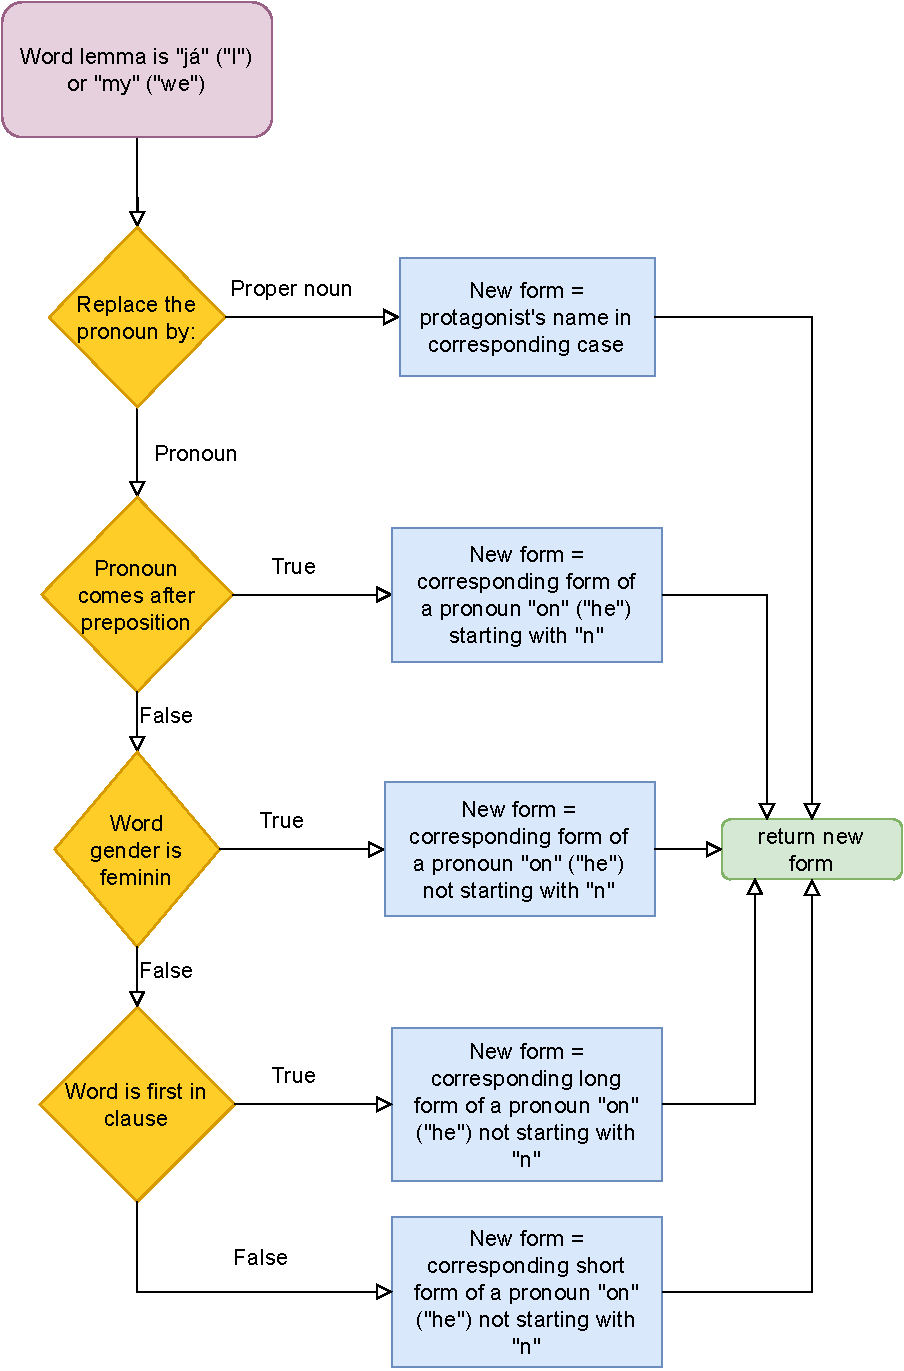
\includegraphics[width=\textwidth]{data/Icher-Perspron-Rule.pdf}
\caption{Personal pronouns replacement rule}
\label{fig:icher-perspron-rule}
\end{figure}

\subsection{Possessive pronouns}

In addition to personal pronouns, possessive pronouns must also be converted. The process is similar to the previous one. The goal is to convert a possessive pronoun \emph{můj (my)} and its forms to possessive pronouns \emph{její (her)} / \emph{jeho (his)}, or the possessive form of a proper noun. Considering the limits given by the morphological analyzer, I have decided not to include the second type of replacement. Therefore all the possessive pronouns would be replaced by possessive pronouns.

The rule is illustrated in a diagram %%\ref{fig:icher-posspron-rule}.

%%\begin{figure}[ht!]
%%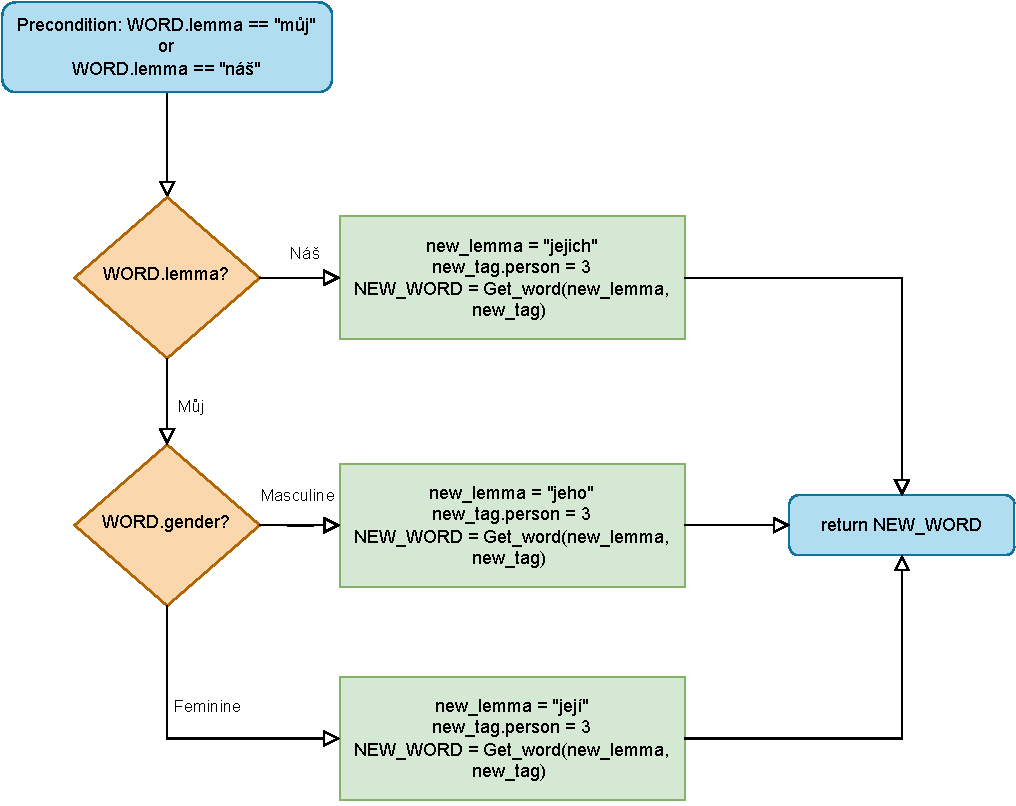
\includegraphics[width=\textwidth]{data/Icher-Posspron-Rule.pdf}
%%\caption{Possessive pronouns replacement rule}
%%\label{fig:icher-posspron-rule}
%%\end{figure}


